\documentclass[withoutpreface,bwprint]{cumcmthesis}

\title{\textbf{skip-gram模型简介}}
\author{2021113140\quad 符世博}
\date{}


\begin{document}
\maketitle
\section{模型介绍}
\subsection{模型概括}
skip-gram模型是由谷歌在2013年提出的用于自然语言处理中的词向量表示模型。网络架构如\cref{fig:1.1}。
其目标为通过给定一个中心词,预测中心词的上下文。为了实现这一目标,skip-gram尝试学习
单词的分布式表示,将单词转换为密集的向量,使得语义相似的单词在向量空间中距离较近。模型输入为
中心词的独热码,输出为上下文的独热码。

\begin{figure}[H]
    \centering
    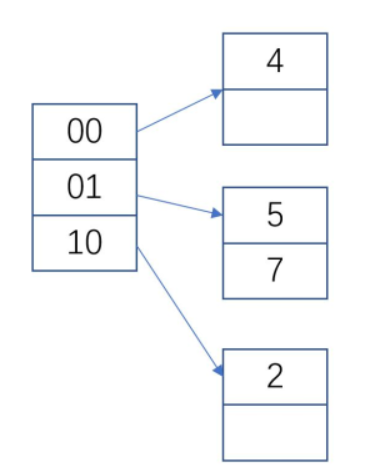
\includegraphics[width=0.55\textwidth]{1}
    \caption{skip-gram模型网络架构}
    \label{fig:1.1}
\end{figure}
\subsection{独热码}
这里简单介绍一下独热码。假设现在有一篇文档,遍历之后发现其一共包含$N$个词,给这$N$个词依次标号
$1,2,3...$。那么独热码就是这样一个$N$维向量,其只有一个位置是$1$,其余位置全为$0$,假设其第
$i$个分量是$1$,那么这个独热码就代表编号为$i$的词。

\subsection{几个重要模型参数}

下面介绍skip-gram模型中的几个重要的参数:
\begin{itemize}
    \item N:嵌入维度;
    \item skip\_window:从当前中心词的两侧侧选取多少个词构成词窗口;
    \item num\_skips:从窗口中选取多少个词作为输出词与中心词构成训练数据。
\end{itemize}

N决定了当前的词会被嵌入到多少维空间中,即用多少维的向量表示一个词。这也是模型架构中输入层到隐含层的
转换矩阵。

skip\_window和num\_skips决定了训练数据是什么样的。以i like eat apple为例,这里取skip\_window=1,
num\_skips=2,中心词为eat。那么从eat的左右两侧各取skip\_window个词,也就是各取1个词构成当前的词窗口['like',
'eat','apple'],之后根据num\_skips从词窗口中选择词作为输出词与当前中心词组成一个训练数据,那么这里组成的训练
数据就是('eat','apple')和('eat','like')。

\subsection{模型训练}

skip-gram模型在训练时:
\begin{itemize}
    \item 隐含层无激活函数;
    \item 输出层采用softmax作为激活函数;
    \item 使用negative sampling作为损失函数。
\end{itemize}

之所以采用softmax作为激活函数,如式\cref{eq:1.1}是因为模型输出是与独热码进行做差,如果不做归一化计算残差效果不是很好。使用
softmax进行归一化后再与独热码计算残差效果会好很多。

\begin{equation}
    s_i=\frac{e^{z_i}}{\sum_1^V{e^{z_j}}}
    \label{eq:1.1}
\end{equation}

采用negative sampling作为损失函数,如式\cref{eq:1.2}而非传统的softmax损失函数的原因是:
\begin{itemize}
    \item 传统的损失函数需要对所有词汇进行计算;
    \item negative sampling通过对负样本进行采样,显著减小计算量。
\end{itemize}

\begin{equation}
    L(\theta)=-\log{(\sigma(V_c\cdot V_\omega))}+\sum_1^k{\log{(\sigma(-V_c\cdot V_{\omega i}))}}
    \label{eq:1.2}
\end{equation}

\subsection{模型应用}

其实输入层到隐含层的权重矩阵$W$的每一行就是对应词的词向量。
那么根据这一矩阵可以将skip-gram模型应用到以下任务中:
\begin{itemize}
    \item 词向量表示:用于词汇相似度计算、词汇聚类、词汇情感分析等任务;
    \item 文档表示:通过将文档中的词汇的词向量进行平均或加权平均,得到整个文档的表示,用于文档相似度计算、文档分类等任务;
    \item 输入特征:词向量可以作为神经网络和其他机器学习模型的输入特征;
    \item 信息检索:词向量可以用于构建词汇的向量空间模型用于信息检索和相关性排序。
\end{itemize}

\section{运行实例}

这里,使用网络上的公开数据集运行skip-gram算法,得到语料中词频top100词的128维词向量表示。将其压缩到2维后进行可视化如
\cref{fig:2.1}

\begin{figure}[H]
    \centering
    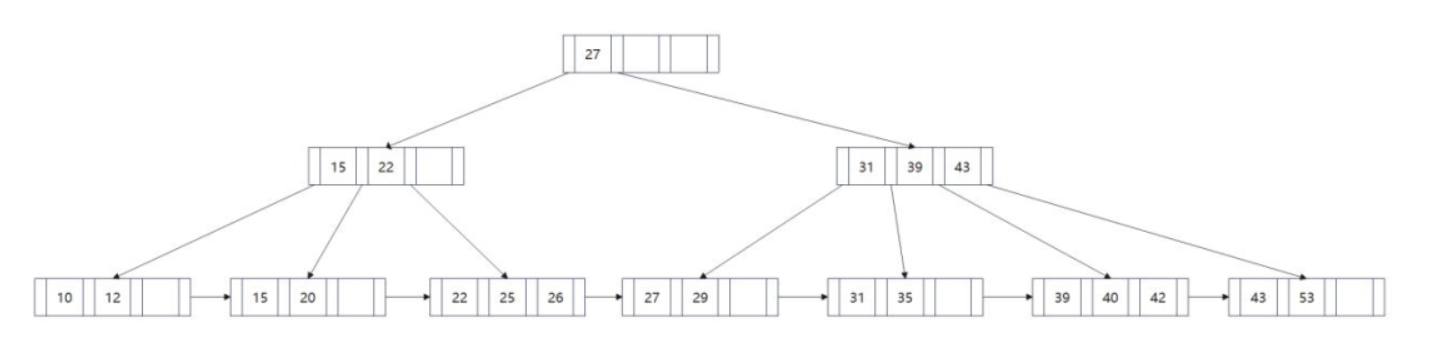
\includegraphics[width=0.85\textwidth]{2}
    \caption{词向量的可视化}
    \label{fig:2.1}
\end{figure}

可以看出,语义相近的词距离更加接近,这也证明了skip-gram算法的可靠性。


\end{document}